\documentclass[12pt,a4paper]{amsart}

\usepackage[slovene]{babel}
\usepackage[utf8]{inputenc}
\usepackage{amsmath,amssymb,amsfonts,bm}
\usepackage{url}
\usepackage{graphicx,subfig}


\textwidth 15cm
\textheight 24cm
\oddsidemargin.5cm
\evensidemargin.5cm
\topmargin-5mm
\addtolength{\footskip}{10pt}
\pagestyle{plain}
\overfullrule=15pt

%%%%%%%%%%%%%%%%%%%%%%%%%%%%%%%%%

%Naslovnica%
\begin{document}
    
\thispagestyle{empty}
\noindent{\large
Univerza v Ljubljani\\[1mm]
Fakulteta za matematiko in fiziko\\[3mm]
Finančna matematika -- 1.~stopnja}
\vfill

\begin{center}{\large
Urška Komatar, Ian Lampič\\[2mm]
{\Huge \bf Intransitive dice}\\[5mm]
Projekt pri predmetu Finančni praktikum\\[1cm]}
\end{center}
\vfill

\noindent{\large
Ljubljana, 2022}
\pagebreak

\section{Opis problema}
Naj bo $p > \frac{1}{2}$ konstanta, A, B in C pa 6 - strane kocke z različnimi števili na svojih straneh, tako da kocka A premaga
B z verjetnostjo vsaj $p$, B premaga C z verjetnostjo vsaj $p$ in C premaga A z verjetnostjo vsaj $p$. Želimo poiskati maksimalni $p$ tako, 
da bo obstajala trojica kock, za katere bo veljala dana lastnost. Kasneje si bova ogledala še primere s štirimi kockami, trostranimi kockami, štiristranimi kockami
in kockami s petimi stranmi.

\section{Način reševanja}
Najprej bova sestavila pomožno funkcijo, ki bo za argumente prejela seznam treh seznamov. V vsakem seznamu bo 6 naravnih števil, ki bodo predstavljale števila na kocki. Če so A, B in C slučajne spremenljivke, ki povedo, koliko pokaže posamezna kocka, bo torej funkcija vračala $min(P(A>B), P(B>C), P(C>A))$. Nato bi naredila krovno funkcijo, ki bi sprejela
naravno število $n$. Znotraj te funkcije bi generirala seznam seznamov z elementi prvih $n$ naravnih števil in na vsakem takem seznamu poklicala pomožno funkcijo.
Medtem bi beležila dobljene verjetnosti in na koncu vrnila maksimum teh vrednosti. Za vsa nadaljna vprašanja bova funkcijo prilagodila danim zahtevam in ponovila postopek.

\section{Primeri netranzitivnih kock}

\subsection{Primer}
\begin{itemize}
    \item A: 2, 2, 6, 6, 7, 7
    \item B: 1, 1, 5, 5, 9, 9
    \item C: 3, 3, 4, 4, 8, 8
\end{itemize}
\begin{align*}
    P(A > B) = P(B > C) = P(C > A) = \frac{5}{9}
\end{align*}
\\Primer, ko je $p=\frac{5}{9}$

\subsection{Efronove kocke}
Efronove kocke so set štirih netranzitivnih kock A, B, C in D z naslednjimi številkami na stranicah:
\begin{itemize}
    \item A: 4, 4, 4, 4, 0, 0
    \item B: 3, 3, 3, 3, 3, 3
    \item C: 6, 6, 2, 2, 2, 2
    \item D: 5, 5, 5, 1, 1, 1
\end{itemize}
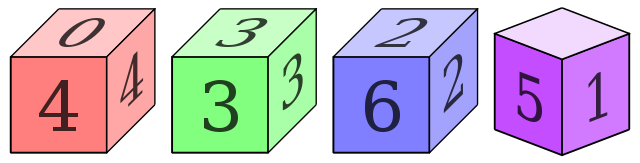
\includegraphics[width=100mm]{Efron's dice.png}
\\Vsaka kocka je premagana s prejšnjo z verjetnostjo $\frac{2}{3}$:
\begin{align*}
   P(A>B) = P(B>C) = P(C>D) = P(D>A) = \frac{2}{3}
\end{align*}
 
B ima na vseh straneh enako število (B je konstantna). A ima 4 od 6 števil višja od B, torej verjetnost da A premaga B je $\frac{2}{3}$, medtem ko
C pa ima 4 od 6 števil manjša od B, torej B premaga C z verjetnostjo $\frac{2}{3}$.
\\$P(C>D)$ izračunamo s seštevanjem pogojnih verjetnosti:
\begin{itemize}
    \item C pokaže 6 ($P = \frac{1}{3}$); premaga D z verjetnostjo 1
    \item C pokaže 2 ($P = \frac{2}{3}$); premaga D le, če D pokaže 1 ($P = \frac{1}{2}$)
\end{itemize}

Torej verjetnost da C premaga D je naslednja:
\begin{align*}
    (\frac{1}{3}\cdot 1)+(\frac{2}{3}\cdot\frac{1}{2}) = \frac{2}{3}
\end{align*}

S podobnim izračunom dobimo še verjetnost, da D premaga A.

 

%%%%%%%%%%%%%%%%%%%%%%%%%%%%%%%%%%%%%%%%
\end{document}